\documentclass[10pt]{article}
\usepackage[margin=1in, paperwidth=8.5in, paperheight=11in]{geometry}
\usepackage{ifpdf,amsmath, amssymb, comment, color, graphicx, stmaryrd,setspace,enumitem,tikz, fancyhdr, wrapfig, textcomp, units, mathptmx, siunitx, pdfpages}
\usepackage[colorlinks]{hyperref}
\usepackage{tikz}
\usetikzlibrary{trees}

\setlength{\headheight}{14.5pt}
\newcommand{\Q}{\mathbb{Q}}
\newcommand{\R}{\mathbb{R}}
\newcommand{\Z}{\mathbb{Z}}
\newcommand{\vu}{\mathbf{u}}
\newcommand{\vv}{\mathbf{v}}
\newcommand{\vw}{\mathbf{w}}
\newcommand{\vi}{\mathbf{i}}
\newcommand{\vj}{\mathbf{j}}
\newcommand{\vk}{\mathbf{k}}
\newcommand{\vn}{\mathbf{n}}
\newcommand{\vr}{\mathbf{r}}
\newcommand{\va}{\mathbf{a}}
\newcommand{\vF}{\mathbf{F}}
\newcommand{\vL}{\mathbf{L}}
\newcommand{\vT}{\mathbf{T}}
\newcommand{\vN}{\mathbf{N}}
\newcommand{\proj}{\operatorname{proj}}
\newcommand{\orth}{\operatorname{orth}}
\newcommand\del\nabla
\newcommand\dotp[1][.5]{\,\mathbin{\vcenter{\hbox{\scalebox{#1}{$\bullet$}}}}\,}

% Solution text is in red. If you want the solutions to show, remove the \iffalse from the definition of the \red command.
%\newcommand{\red}[1]{ %\iffalse
%	\textcolor{red}{#1} }%\fi}

\newenvironment{red}{\color{red}}{\ignorespacesafterend}
\newcommand{\blue}[1]{\textcolor{blue}{#1}}
\newcommand{\green}[1]{\textcolor{green}{#1}}
\renewcommand{\section}[1]{\begin{center} \textbf{#1} \\\end{center}}
%
\hyphenpenalty=5000
\setlength{\parindent}{0in}
%\oddsidemargin=-.25in
\allowdisplaybreaks
\pagestyle{fancy}
\renewcommand{\headrulewidth}{0pt}
\lhead{MATH 203}
\rhead{Fall 2019}
%\lfoot{\copyright\ CLEAR Calculus 2010}
\cfoot{}

\begin{document}
%


%\onehalfspacing
\allowdisplaybreaks
%##################################################################
\section{PS\#9 -- Optimization and Lagrange multipliers - \red{Answer key} }

\begin{enumerate}[leftmargin=0pt]
    
    \item (AC Multi 2.7 \#18) If a continuous function $f$ of a \textbf{single variable} has two critical numbers $c_1$ and $c_2$ at which $f$ has relative maximum values, then $f$ must have another critical number $c_3$, because ``it is impossible to have two mountains without some sort of valley in between. The other critical point can be a saddle point (a pass between the mountains) or a local minimum (a true valley).'' (From Calculus in Vector Spaces by Lawrence J. Corwin and Robert H. Szczarb.)
    
    Consider the function $f$ defined by $f(x,y) = 4x^2e^y -2x^4 -e^{4y}.$ (From Ira Rosenholz in the Problems Section of the Mathematics Magazine, Vol. 60 NO. 1, February 1987.) \textbf{Note:} This is a function of two variables, so it doesn't have to follow the rule outlined in the previous paragraph.
    
    Show that $f$ has exactly two critical points, and that $f$ has relative maximum values at each of these critical points. 
    
    \begin{red}
    So we're looking for zeroes of the gradient.
    \begin{align*}
        \del f &= \langle f_x(x, y), f_y(x,y) \rangle \\
        &= \langle 8x e^y - 8x^3, 4x^2 e^y - 4e^{4y} \rangle
        \\
        \intertext{Let's focus on the first component:}
        0 &= 8x e^y - 8x^3 = 8x(e^y - x^2) \\
        \intertext{So, either $x = 0$ or $e^y = x^2$. Note that $x=0$ is not going to make the second component zero, so we can discard it. From the second component,}
        0 &= 4x^2 e^y - 4e^{4y} = 4e^y (x^2 - e^{3y}) \\
        \intertext{So, either $e^y = 0$, which it never does, or $x^2 = e^{3y}$. Therefore, I've got two things that both have to be equal to $x^2$, so they must equal each other:}
        e^y &= e^{3y} \\
        y &= 3y \textrm{, so } y = 0 \\
        \intertext{Therefore, }
        x^2 &= e^0 = 1 \textrm{, so } x = \pm 1
    \end{align*}
    So, we have precisely two critical points: $(1, 0)$ and $(-1, 0)$. Let's use the discriminant to classify them. We need to calculate our second partials:
    \[
    \begin{array}{ll}
       f_{xx} = 8e^y-24x^2  & f_{yx} = 8xe^y \\
       f_{xy} = 8xe^y  & f_{yy} = 4x^2 e^y-16 e^{4y}
    \end{array}
    \]
    At the critical point $(1, 0)$:
    \[
    \begin{array}{ll}
        f_{xx} = 8e^0-24(1)^2 = -16 & f_{yx} = 8(1)e^0 = 8 \\
        f_{xy} = 8(1)e^0 = 8 & f_{yy} = 4(1)^2 e^0 - 16 e^0 = -12
    \end{array}
    \]
    So $D = (-16)(-12) - 8^2 = 128 > 0$, and $f_{xx} < 0$, so this is a maximum.
    
    At the critical point $(-1, 0)$:
    \[
    \begin{array}{ll}
        f_{xx} = 8e^0-24(-1)^2 = -16 & f_{yx} = 8(-1)e^0 = -8 \\
        f_{xy} = 8(1)e^0 = -8 & f_{yy} = 4(1)^2 e^0 - 16 e^0 = -12
    \end{array}
    \]
    So $D = (-16)(-12) - (-8)^2 = 128 > 0$, and $f_{xx} < 0$, so this is a maximum.
    \end{red}
    \pagebreak
    
    Explain how this function $f$ illustrates that it really is possible to have two mountains without some sort of valley in between. Use appropriate technology to draw the surface defined by $f$ to see graphically how this happens.
    
    \begin{red}
    Yeah, so \href{https://www.monroecc.edu/faculty/paulseeburger/calcnsf/CalcPlot3D/?type=z;z=4x^2e^y-2x^4-e^(4y);visible=true;umin=-2;umax=2;vmin=-2;vmax=2;grid=50;format=normal;alpha=-1;constcol=rgb(255,0,0);view=0;contourcolor=red;fixdomain=false&type=window;hsrmode=3;nomidpts=true;anaglyph=-1;center=2.507369696231452,8.657081705234903,4.332208854072867,1;focus=0,0,0,1;up=-0.3279946341240409,-0.34507444582480573,0.8793993102251901,1;transparent=false;alpha=140;twoviews=false;unlinkviews=false;axisextension=0.7;xaxislabel=x;yaxislabel=y;zaxislabel=z;edgeson=true;faceson=true;showbox=true;showaxes=true;showticks=true;perspective=true;centerxpercent=0.5;centerypercent=0.5;rotationsteps=30;autospin=true;xygrid=false;yzgrid=false;xzgrid=false;gridsonbox=true;gridplanes=false;gridcolor=rgb(128,128,128);xmin=-2;xmax=2;ymin=-2;ymax=2;zmin=-2;zmax=2;xscale=1;yscale=1;zscale=1;zcmin=-4;zcmax=4;zoom=0.886667;xscalefactor=1;yscalefactor=1;zscalefactor=1}{check this function out} (that's clickable and takes you to CalcPlot3D):
    
    \begin{center}
        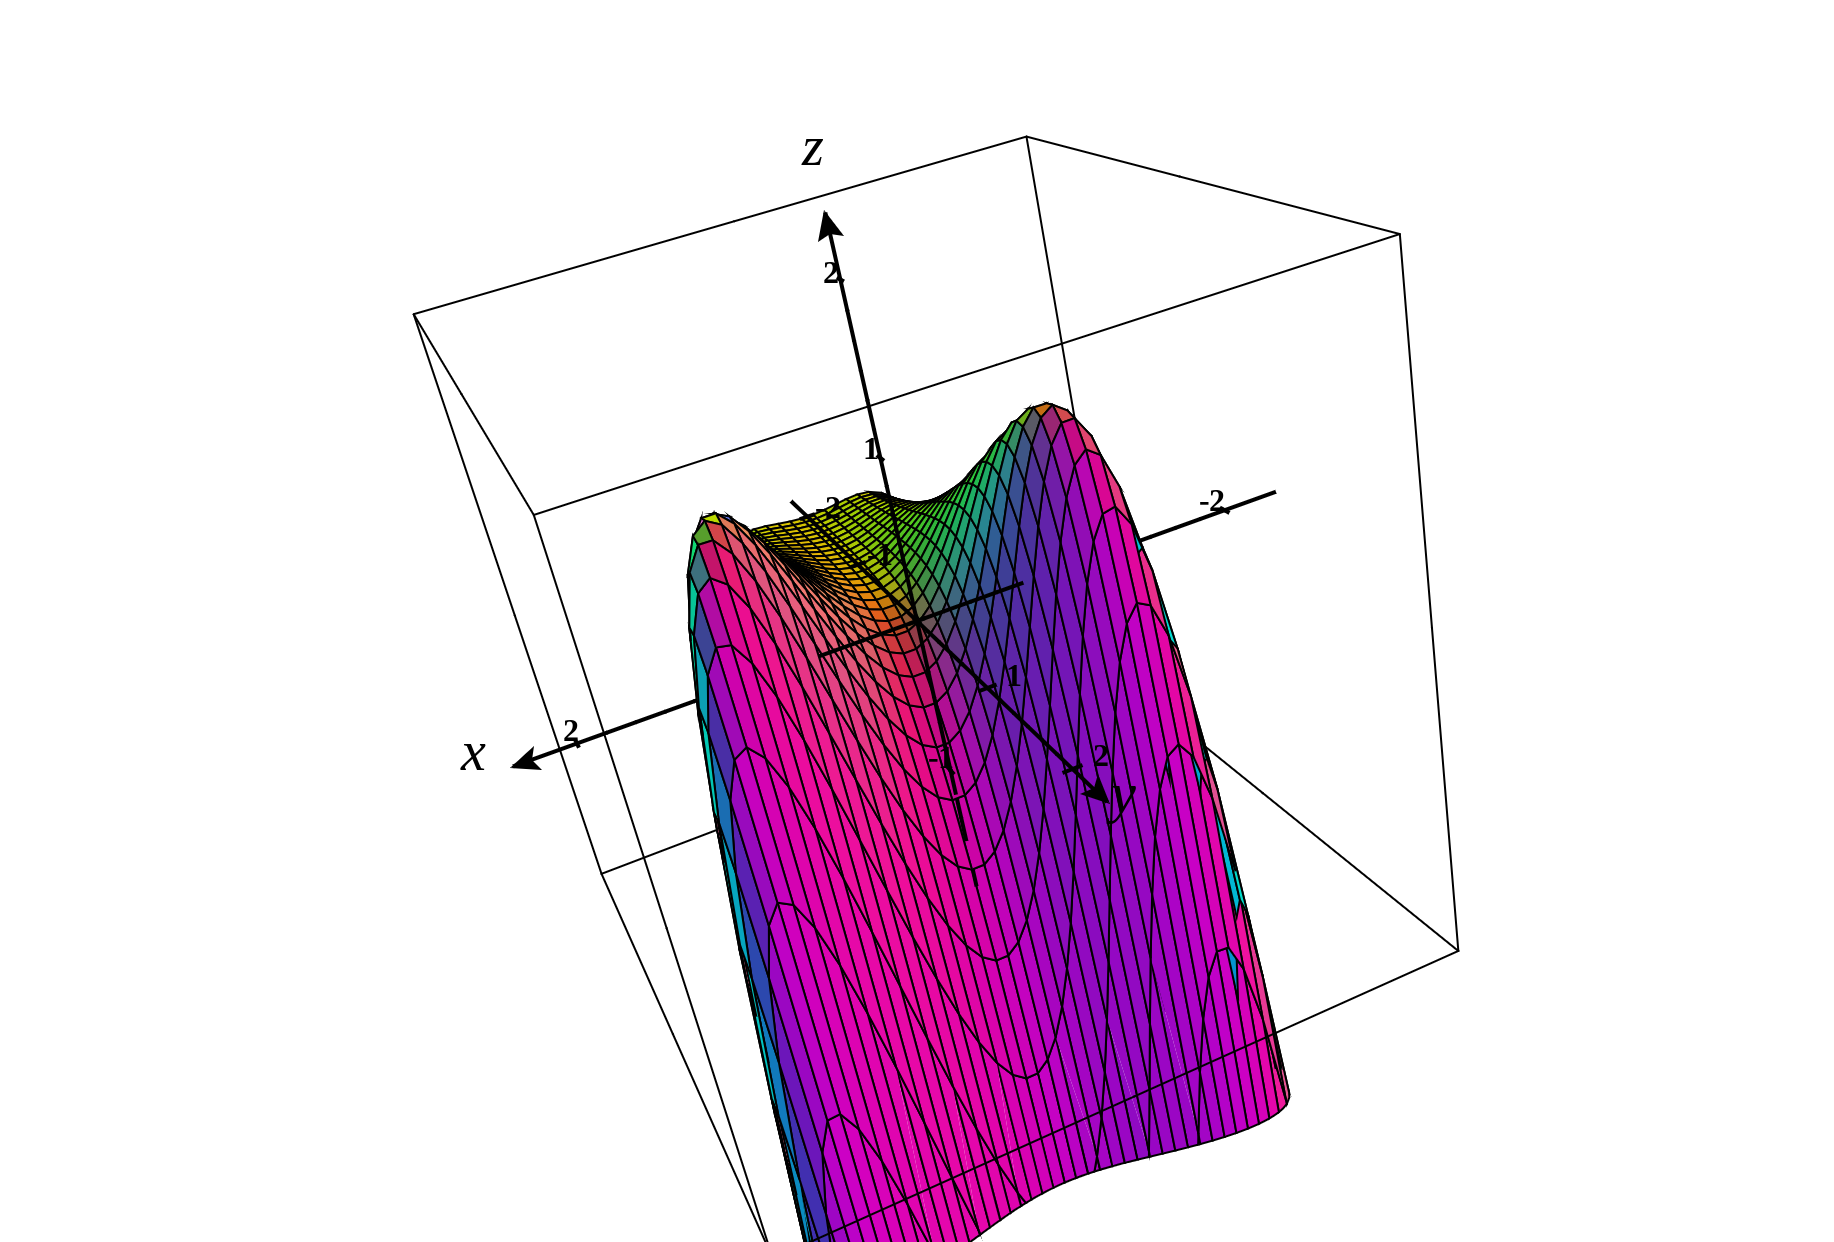
\includegraphics[width=0.75\textwidth]{CalcPlot3D-plot.png}
    \end{center}
    
    So there kind of \textbf{is} a valley between the two mountains, but there's no point at the bottom of the valley, because the valley just continues down forever without ever hitting a critical point.
    \end{red}
    
    \item The Cobb-Douglas production function is used in economics to model production levels based on labor and equipment. Suppose we have a specific Cobb-Douglas function of the form \[f(x, y) = 50 x^{0.4}y^{0.6},\] where $x$ is the dollar amount spent on labor and $y$ the dollar amount spent on equipment. Use the method of Lagrange multipliers to determine how much should be spent on labor and how much on equipment to maximize productivity if we have a total of \$1.5 million dollars to invest in labor and equipment.
    
    \begin{red}
    The method of Lagrange multipliers needs us to have a constraint. Here the constraint is the total amount of money:
    \[x + y = 1.5 \textrm{ million}.\]
    So, our $f$ is the function given in the problem, our $g(x,y) = x+y = 1.5$. Off we go to Lagrange mulitpliers land. We need to calculate the gradients: 
    \begin{align*}
        \del f &= \langle 20 x^{-0.6} y^{0.6}, 30 x^{0.4} y^{-0.4} \rangle \\
        \del g &= \langle 1, 1 \rangle
        \intertext{So, setting up $\del f = \lambda \del g$ together with our constraint:}
        20 x^{-0.6} y^{0.6} &= \lambda\cdot 1 \\
        30 x^{0.4} y^{-0.4} &= \lambda\cdot 1 \\
        x+y &= 1.5
        \intertext{It's nice that we have two things that both equal $\lambda$, so they must just equal each other. Also, our constraint tells us that $y=1.5-x$:}
        20 x^{-0.6} (1.5-x)^{0.6} &= 30 x^{0.4} (1.5-x)^{-0.4} \\
        20\frac{(1.5-x)^{0.6}}{x^{0.6}} &= 30 \frac{x^{0.4}}{(1.5-x)^{0.4}}
        \intertext{Clear denominators. It's so nice that the powers add up to 1, eh?}
        20 (1.5-x)^{0.6} (1.5-x)^{0.4} &= 30 x^{0.4} x^{0.6} \\
        20 (1.5-x) &= 30 x \\
        30 - 20x &= 30x \\
        30 &= 50x \\
        x = 0.6; &\quad y = 0.9
    \end{align*}
    So we should spend $\$600,000$ on labor and $\$900,000$ on equipment.
    \end{red}
    \end{enumerate}

\begin{red}
\textbf{Learning Targets Reflection:} Maybe some HBTs, S1, D9*, D11, D12, maybe others.

(See bonus problem on next page.)
\end{red}

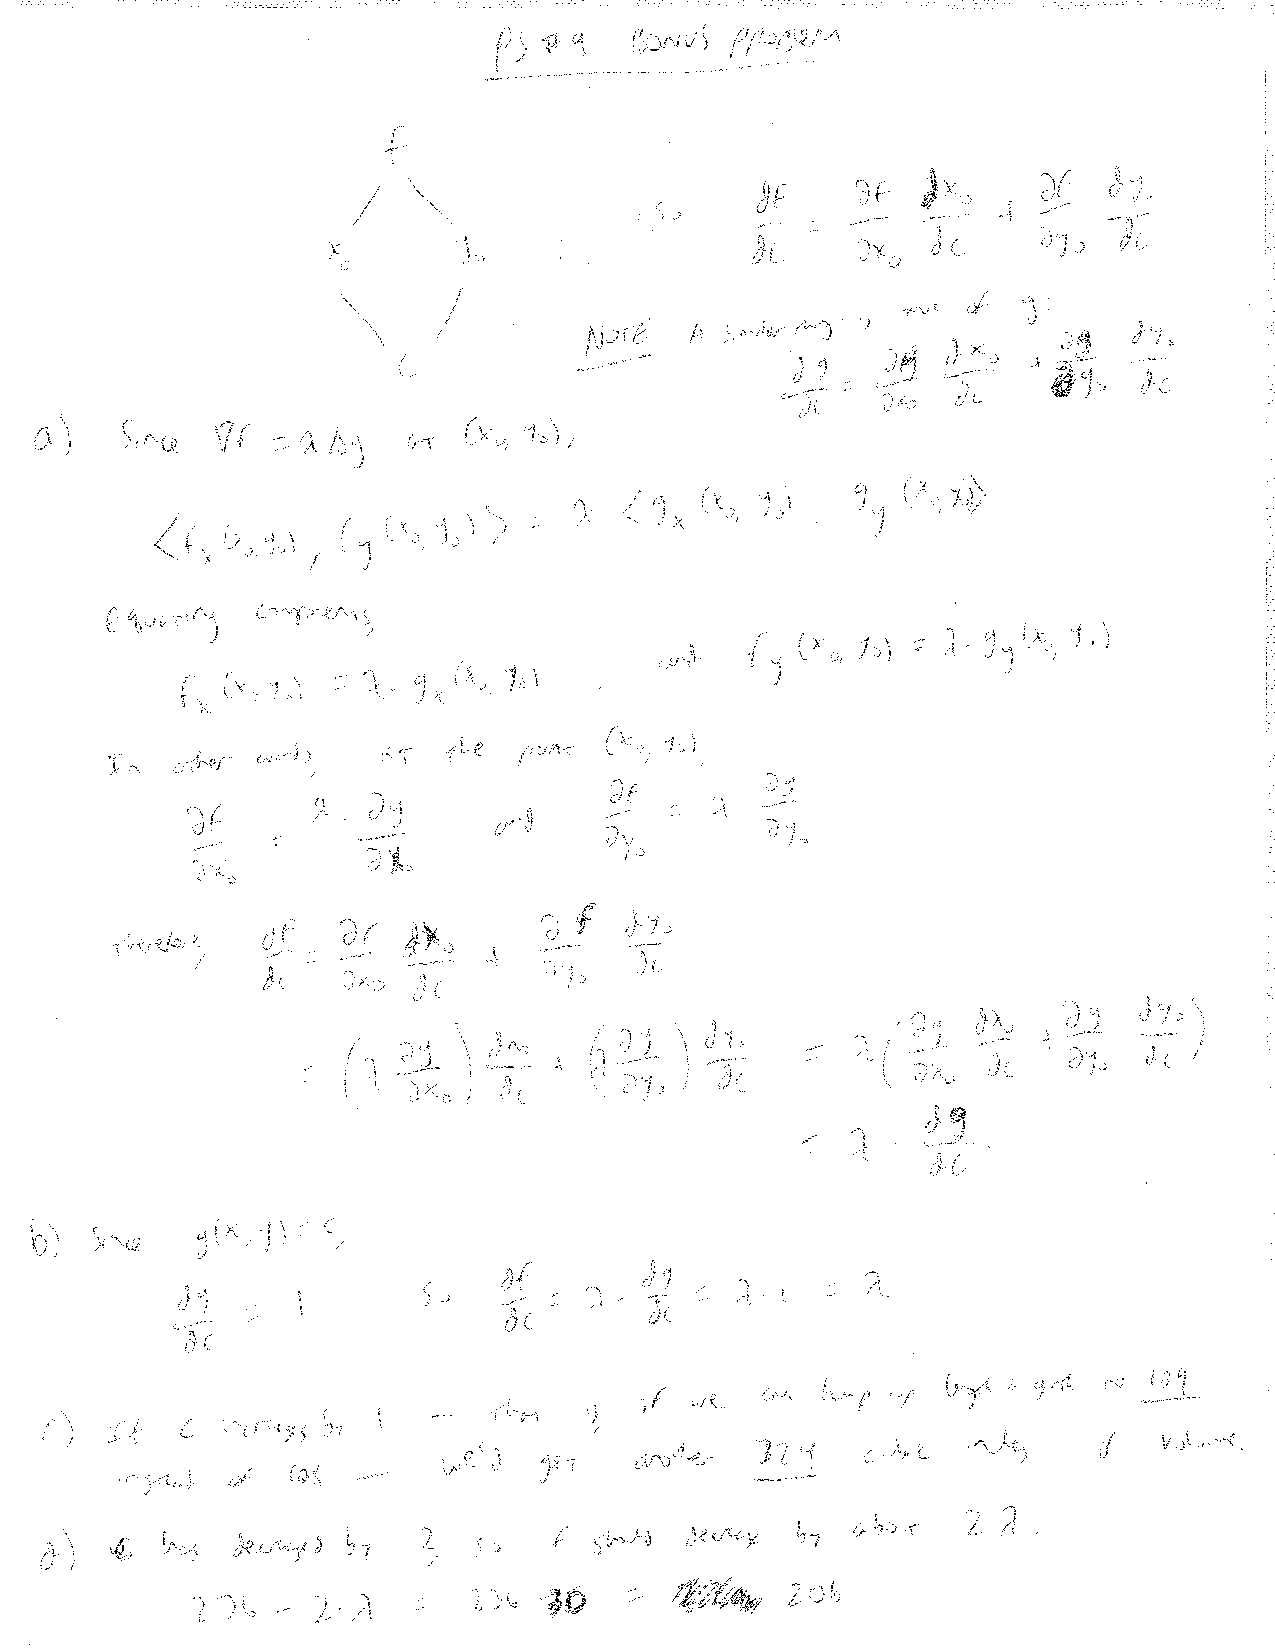
\includepdf[pages=-]{ps-9-bonus.pdf}

\end{document}